\section{CRange\-Error  Class Reference}
\label{classCRangeError}\index{CRangeError@{CRange\-Error}}
{\tt \#include $<$CRange\-Error.h$>$}

Inheritance diagram for CRange\-Error::\begin{figure}[H]
\begin{center}
\leavevmode
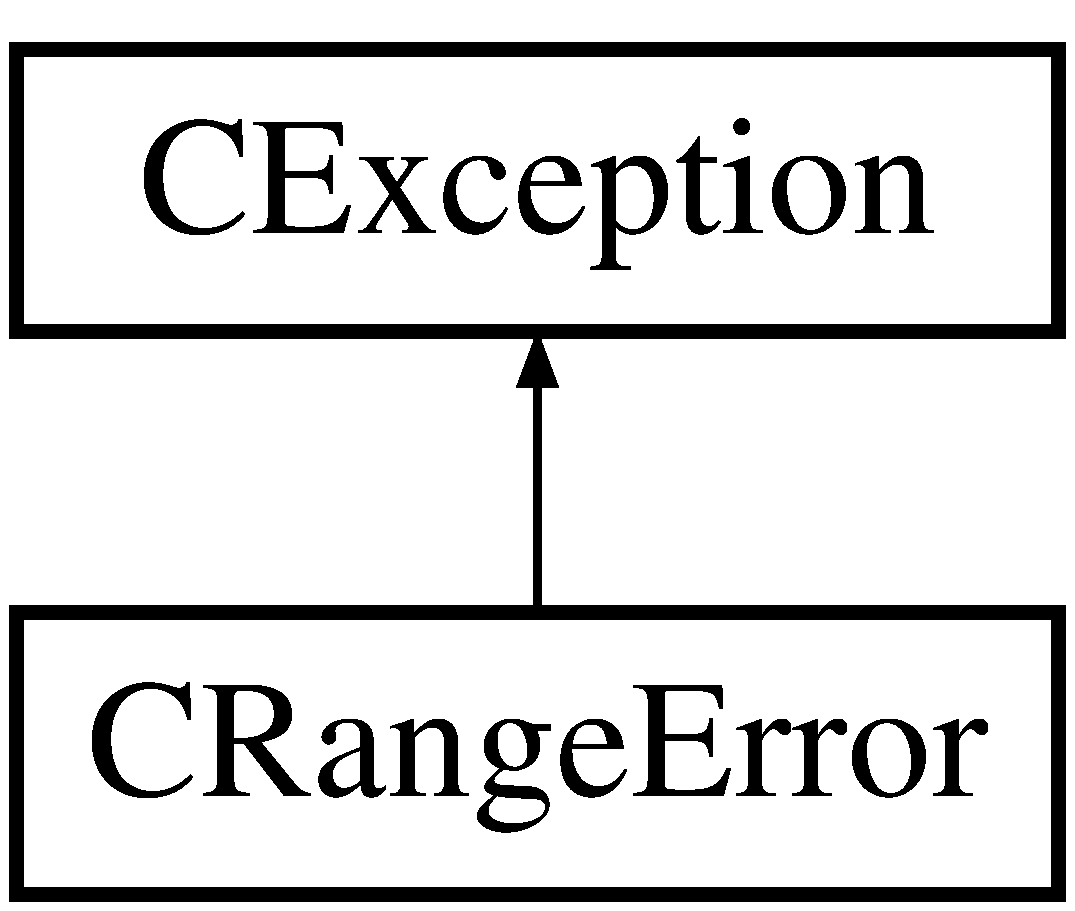
\includegraphics[height=2cm]{classCRangeError}
\end{center}
\end{figure}
\subsection*{Public Types}
\begin{CompactItemize}
\item 
enum \{ {\bf kn\-Too\-Low}, 
{\bf kn\-Too\-High}
 \}
\end{CompactItemize}
\subsection*{Public Methods}
\begin{CompactItemize}
\item 
{\bf CRange\-Error} ({\bf Int\_\-t} n\-Low, {\bf Int\_\-t} n\-High, {\bf Int\_\-t} n\-Requested, const char $\ast$p\-Doing)
\item 
{\bf CRange\-Error} ({\bf Int\_\-t} n\-Low, {\bf Int\_\-t} n\-High, {\bf Int\_\-t} n\-Requested, const string \&r\-Doing)
\item 
virtual {\bf $\sim$CRange\-Error} ()
\item 
{\bf CRange\-Error} (const CRange\-Error \&a\-CRange\-Error)
\item 
CRange\-Error {\bf operator=} (const CRange\-Error \&a\-CRange\-Error)
\item 
int {\bf operator==} (const CRange\-Error \&a\-CRange\-Error)
\item 
{\bf Int\_\-t} {\bf get\-Low} () const
\item 
{\bf Int\_\-t} {\bf get\-High} () const
\item 
{\bf Int\_\-t} {\bf get\-Requested} () const
\item 
virtual const char $\ast$ {\bf Reason\-Text} () const
\item 
virtual {\bf Int\_\-t} {\bf Reason\-Code} () const
\end{CompactItemize}
\subsection*{Protected Methods}
\begin{CompactItemize}
\item 
void {\bf set\-Low} ({\bf Int\_\-t} am\_\-n\-Low)
\item 
void {\bf set\-High} ({\bf Int\_\-t} am\_\-n\-High)
\item 
void {\bf set\-Requested} ({\bf Int\_\-t} am\_\-n\-Requested)
\item 
void {\bf Update\-Reason} ()
\end{CompactItemize}
\subsection*{Private Attributes}
\begin{CompactItemize}
\item 
{\bf Int\_\-t} {\bf m\_\-n\-Low}
\item 
{\bf Int\_\-t} {\bf m\_\-n\-High}
\item 
{\bf Int\_\-t} {\bf m\_\-n\-Requested}
\item 
string {\bf m\_\-Reason\-Text}
\end{CompactItemize}


\subsection{Member Enumeration Documentation}
\subsubsection{\setlength{\rightskip}{0pt plus 5cm}anonymous enum}\label{classCRangeError_s2}


\begin{Desc}
\item[Enumeration values:]\par
\begin{description}
\index{knTooLow@{knTooLow}!CRangeError@{CRange\-Error}}\index{CRangeError@{CRangeError}!knTooLow@{kn\-Too\-Low}}\item[{\em 
{\em kn\-Too\-Low}\label{classCRangeError_s2s0}
}]\index{knTooHigh@{knTooHigh}!CRangeError@{CRange\-Error}}\index{CRangeError@{CRangeError}!knTooHigh@{kn\-Too\-High}}\item[{\em 
{\em kn\-Too\-High}\label{classCRangeError_s2s1}
}]\end{description}
\end{Desc}



Definition at line 315 of file CRange\-Error.h.

\subsection{Constructor \& Destructor Documentation}
\index{CRangeError@{CRange\-Error}!CRangeError@{CRangeError}}
\index{CRangeError@{CRangeError}!CRangeError@{CRange\-Error}}
\subsubsection{\setlength{\rightskip}{0pt plus 5cm}CRange\-Error::CRange\-Error ({\bf Int\_\-t} {\em n\-Low}, {\bf Int\_\-t} {\em n\-High}, {\bf Int\_\-t} {\em n\-Requested}, const char $\ast$ {\em p\-Doing})\hspace{0.3cm}{\tt  [inline]}}\label{classCRangeError_a0}




Definition at line 321 of file CRange\-Error.h.

References Int\_\-t, m\_\-n\-High, m\_\-n\-Low, m\_\-n\-Requested, and Update\-Reason().\index{CRangeError@{CRange\-Error}!CRangeError@{CRangeError}}
\index{CRangeError@{CRangeError}!CRangeError@{CRange\-Error}}
\subsubsection{\setlength{\rightskip}{0pt plus 5cm}CRange\-Error::CRange\-Error ({\bf Int\_\-t} {\em n\-Low}, {\bf Int\_\-t} {\em n\-High}, {\bf Int\_\-t} {\em n\-Requested}, const string \& {\em r\-Doing})\hspace{0.3cm}{\tt  [inline]}}\label{classCRangeError_a1}




Definition at line 328 of file CRange\-Error.h.

References Int\_\-t, m\_\-n\-High, m\_\-n\-Low, m\_\-n\-Requested, and Update\-Reason().\index{CRangeError@{CRange\-Error}!~CRangeError@{$\sim$CRangeError}}
\index{~CRangeError@{$\sim$CRangeError}!CRangeError@{CRange\-Error}}
\subsubsection{\setlength{\rightskip}{0pt plus 5cm}virtual CRange\-Error::$\sim$CRange\-Error ()\hspace{0.3cm}{\tt  [inline, virtual]}}\label{classCRangeError_a2}




Definition at line 335 of file CRange\-Error.h.\index{CRangeError@{CRange\-Error}!CRangeError@{CRangeError}}
\index{CRangeError@{CRangeError}!CRangeError@{CRange\-Error}}
\subsubsection{\setlength{\rightskip}{0pt plus 5cm}CRange\-Error::CRange\-Error (const CRange\-Error \& {\em a\-CRange\-Error})\hspace{0.3cm}{\tt  [inline]}}\label{classCRangeError_a3}




Definition at line 339 of file CRange\-Error.h.

References m\_\-n\-High, m\_\-n\-Low, m\_\-n\-Requested, and Update\-Reason().

\subsection{Member Function Documentation}
\index{CRangeError@{CRange\-Error}!getHigh@{getHigh}}
\index{getHigh@{getHigh}!CRangeError@{CRange\-Error}}
\subsubsection{\setlength{\rightskip}{0pt plus 5cm}{\bf Int\_\-t} CRange\-Error::get\-High () const\hspace{0.3cm}{\tt  [inline]}}\label{classCRangeError_a7}




Definition at line 384 of file CRange\-Error.h.

References Int\_\-t, and m\_\-n\-High.\index{CRangeError@{CRange\-Error}!getLow@{getLow}}
\index{getLow@{getLow}!CRangeError@{CRange\-Error}}
\subsubsection{\setlength{\rightskip}{0pt plus 5cm}{\bf Int\_\-t} CRange\-Error::get\-Low () const\hspace{0.3cm}{\tt  [inline]}}\label{classCRangeError_a6}




Definition at line 380 of file CRange\-Error.h.

References Int\_\-t, and m\_\-n\-Low.\index{CRangeError@{CRange\-Error}!getRequested@{getRequested}}
\index{getRequested@{getRequested}!CRangeError@{CRange\-Error}}
\subsubsection{\setlength{\rightskip}{0pt plus 5cm}{\bf Int\_\-t} CRange\-Error::get\-Requested () const\hspace{0.3cm}{\tt  [inline]}}\label{classCRangeError_a8}




Definition at line 388 of file CRange\-Error.h.

References Int\_\-t, and m\_\-n\-Requested.\index{CRangeError@{CRange\-Error}!operator=@{operator=}}
\index{operator=@{operator=}!CRangeError@{CRange\-Error}}
\subsubsection{\setlength{\rightskip}{0pt plus 5cm}CRange\-Error CRange\-Error::operator= (const CRange\-Error \& {\em a\-CRange\-Error})\hspace{0.3cm}{\tt  [inline]}}\label{classCRangeError_a4}




Definition at line 350 of file CRange\-Error.h.

References m\_\-n\-High, m\_\-n\-Low, m\_\-n\-Requested, CException::operator=(), and Update\-Reason().\index{CRangeError@{CRange\-Error}!operator==@{operator==}}
\index{operator==@{operator==}!CRangeError@{CRange\-Error}}
\subsubsection{\setlength{\rightskip}{0pt plus 5cm}int CRange\-Error::operator== (const CRange\-Error \& {\em a\-CRange\-Error})\hspace{0.3cm}{\tt  [inline]}}\label{classCRangeError_a5}




Definition at line 365 of file CRange\-Error.h.

References m\_\-n\-High, m\_\-n\-Low, m\_\-n\-Requested, and CException::operator==().\index{CRangeError@{CRange\-Error}!ReasonCode@{ReasonCode}}
\index{ReasonCode@{ReasonCode}!CRangeError@{CRange\-Error}}
\subsubsection{\setlength{\rightskip}{0pt plus 5cm}{\bf Int\_\-t} CRange\-Error::Reason\-Code () const\hspace{0.3cm}{\tt  [virtual]}}\label{classCRangeError_a10}


Returns a code which describes the reason for the exception . This is exception type specific and may be used to do detailed exception analysis and recovery. For example in the {\bf CErrno\-Exception} {\rm (p.\,\pageref{classCErrnoException})} class, the errno at the time of instantiation of the object is returned. The default returns -1 

Reimplemented from {\bf CException} {\rm (p.\,\pageref{classCException_a9})}.

Definition at line 334 of file CRange\-Error.cpp.

References kn\-Too\-High, kn\-Too\-Low, m\_\-n\-High, m\_\-n\-Low, and m\_\-n\-Requested.\index{CRangeError@{CRange\-Error}!ReasonText@{ReasonText}}
\index{ReasonText@{ReasonText}!CRangeError@{CRange\-Error}}
\subsubsection{\setlength{\rightskip}{0pt plus 5cm}const char $\ast$ CRange\-Error::Reason\-Text () const\hspace{0.3cm}{\tt  [virtual]}}\label{classCRangeError_a9}


Returns a const pointer to text which describes the reason the exception was thrown. This is exception type specific. The default action returns a pointer to the constant string: \char`\"{}Unspecified Exception\char`\"{} 

Reimplemented from {\bf CException} {\rm (p.\,\pageref{classCException_a8})}.

Definition at line 316 of file CRange\-Error.cpp.

References m\_\-Reason\-Text.\index{CRangeError@{CRange\-Error}!setHigh@{setHigh}}
\index{setHigh@{setHigh}!CRangeError@{CRange\-Error}}
\subsubsection{\setlength{\rightskip}{0pt plus 5cm}void CRange\-Error::set\-High ({\bf Int\_\-t} {\em am\_\-n\-High})\hspace{0.3cm}{\tt  [inline, protected]}}\label{classCRangeError_b1}




Definition at line 400 of file CRange\-Error.h.

References Int\_\-t, m\_\-n\-High, and Update\-Reason().\index{CRangeError@{CRange\-Error}!setLow@{setLow}}
\index{setLow@{setLow}!CRangeError@{CRange\-Error}}
\subsubsection{\setlength{\rightskip}{0pt plus 5cm}void CRange\-Error::set\-Low ({\bf Int\_\-t} {\em am\_\-n\-Low})\hspace{0.3cm}{\tt  [inline, protected]}}\label{classCRangeError_b0}




Definition at line 395 of file CRange\-Error.h.

References Int\_\-t, m\_\-n\-Low, and Update\-Reason().\index{CRangeError@{CRange\-Error}!setRequested@{setRequested}}
\index{setRequested@{setRequested}!CRangeError@{CRange\-Error}}
\subsubsection{\setlength{\rightskip}{0pt plus 5cm}void CRange\-Error::set\-Requested ({\bf Int\_\-t} {\em am\_\-n\-Requested})\hspace{0.3cm}{\tt  [inline, protected]}}\label{classCRangeError_b2}




Definition at line 405 of file CRange\-Error.h.

References Int\_\-t, m\_\-n\-Requested, and Update\-Reason().\index{CRangeError@{CRange\-Error}!UpdateReason@{UpdateReason}}
\index{UpdateReason@{UpdateReason}!CRangeError@{CRange\-Error}}
\subsubsection{\setlength{\rightskip}{0pt plus 5cm}void CRange\-Error::Update\-Reason ()\hspace{0.3cm}{\tt  [protected]}}\label{classCRangeError_b3}




Definition at line 363 of file CRange\-Error.cpp.

References m\_\-n\-High, m\_\-n\-Low, m\_\-n\-Requested, and m\_\-Reason\-Text.

Referenced by CRange\-Error(), operator=(), set\-High(), set\-Low(), and set\-Requested().

\subsection{Member Data Documentation}
\index{CRangeError@{CRange\-Error}!m_nHigh@{m\_\-nHigh}}
\index{m_nHigh@{m\_\-nHigh}!CRangeError@{CRange\-Error}}
\subsubsection{\setlength{\rightskip}{0pt plus 5cm}{\bf Int\_\-t} CRange\-Error::m\_\-n\-High\hspace{0.3cm}{\tt  [private]}}\label{classCRangeError_o1}




Definition at line 307 of file CRange\-Error.h.

Referenced by CRange\-Error(), get\-High(), operator=(), operator==(), Reason\-Code(), set\-High(), and Update\-Reason().\index{CRangeError@{CRange\-Error}!m_nLow@{m\_\-nLow}}
\index{m_nLow@{m\_\-nLow}!CRangeError@{CRange\-Error}}
\subsubsection{\setlength{\rightskip}{0pt plus 5cm}{\bf Int\_\-t} CRange\-Error::m\_\-n\-Low\hspace{0.3cm}{\tt  [private]}}\label{classCRangeError_o0}




Definition at line 306 of file CRange\-Error.h.

Referenced by CRange\-Error(), get\-Low(), operator=(), operator==(), Reason\-Code(), set\-Low(), and Update\-Reason().\index{CRangeError@{CRange\-Error}!m_nRequested@{m\_\-nRequested}}
\index{m_nRequested@{m\_\-nRequested}!CRangeError@{CRange\-Error}}
\subsubsection{\setlength{\rightskip}{0pt plus 5cm}{\bf Int\_\-t} CRange\-Error::m\_\-n\-Requested\hspace{0.3cm}{\tt  [private]}}\label{classCRangeError_o2}




Definition at line 308 of file CRange\-Error.h.

Referenced by CRange\-Error(), get\-Requested(), operator=(), operator==(), Reason\-Code(), set\-Requested(), and Update\-Reason().\index{CRangeError@{CRange\-Error}!m_ReasonText@{m\_\-ReasonText}}
\index{m_ReasonText@{m\_\-ReasonText}!CRangeError@{CRange\-Error}}
\subsubsection{\setlength{\rightskip}{0pt plus 5cm}string CRange\-Error::m\_\-Reason\-Text\hspace{0.3cm}{\tt  [private]}}\label{classCRangeError_o3}




Definition at line 310 of file CRange\-Error.h.

Referenced by Reason\-Text(), and Update\-Reason().

The documentation for this class was generated from the following files:\begin{CompactItemize}
\item 
{\bf CRange\-Error.h}\item 
{\bf CRange\-Error.cpp}\end{CompactItemize}
